\documentclass[compress]{beamer}
\usepackage{mvppdbPresentation}
\title[Representation Learning]{GCCA}
\author[]{Pushpendre Rastogi}
\date[]{}
\subject{GCCA}
\newcommand{\fcite}[1]{{\tiny(Source: #1)}\\}
\newcommand{\Cov}{\textrm{Cov}}
\def \bZ{\textbf{Z}}
\def \bC{\textbf{C}}
\usepackage{tikz}
\usetikzlibrary{bayesnet}
\usetikzlibrary{positioning}
\usepackage[all]{xy}
\usepackage{caption}
\usepackage{subcaption}
\usepackage{pifont}
\usepackage[table]{xcolor}
%\usepackage{color, colortbl}
%% \newcommand{\cwindow}{1, 2, 4, 6, 8, 10, 12, 14, 15}
%% \newcommand{\cwinlen}{9}
%% \newcommand{\ctotalview}{16}
%\newcommand{\xline}[0]{\noindent\underline{\makebox[0.1cm][l]{}}}
\newcommand{\specialcell}[2][c]{\begin{tabular}[#1]{@{}c@{}}#2\end{tabular}}
\usepackage{array}
\newcolumntype{H}{>{\setbox0=\hbox\bgroup}c<{\egroup}@{}}
\makeatletter
\newcommand{\remove}[1]{#1}
\newcommand*{\@rowstyle}{}

\newcommand*{\rowstyle}[1]{% sets the style of the next row
  \gdef\@rowstyle{#1}%
  \@rowstyle\ignorespaces%
}

\newcolumntype{=}{% resets the row style
  >{\gdef\@rowstyle{}}%
}

\newcolumntype{+}{% adds the current row style to the next column
  >{\@rowstyle}%
}

\definecolor{lightgray}{gray}{0.9}
\definecolor{darkgray}{gray}{0.7}
\definecolor{darkergray}{gray}{0.5}

%\usepackage[utf8]{inputenc}
%%%%%%%%%%% BEGIN DOCUMENT
\begin{document}
\frame{\titlepage}

%%
\begin{frame}{Interpretations Of GCCA - Maximize Measure}
  \fcite{Kettenring, 1979, Canonical analysis of several sets of variables.}
    
  Suppose you have $m$ sets of varibles
  $$(X_1, \ldots, \; X_m) : X_i \in \mathbb{R}^{d_i}$$

  In GCCA we find ``Linear functionals''/Directions/Vectors $L_i$
  $$(L_1,  \ldots, \; L_m)$$
  With the constraint that the projections $Z_i$ have unit variance.
  $$Z_i = L_i^\top X_i : \textrm{var}(Z_i) = 1$$
  Choose $L_i \; \forall i \in [1, \ldots, \; m]$ so as to
  maximize some measure of the matrix $\Phi$ containing the correlation(covariance)
  coeffcients of $Z_i$.
\end{frame}

\begin{frame}{Interpretations of GCCA - Maximize Measure}
    \fcite{Kettenring, 1979, Canonical analysis of several sets of
      variables.}
    
   Depending on the function optimized we get  different types of GCCA.
  \begin{description}
  \item[SUMCOR] max(sum(sum($\Phi$)))
  \item [MAXVAR] max($||\Phi||_2$)
  \item [SSQCOR] max($||\Phi||_f$)
  \item [MINVAR] min($\lambda_{\min}$) where $\lambda$
    denotes eigenvalues of $\Phi$
  \item [GENVAR] minimize($\Pi \, \lambda_i$)
  \end{description}
  
\end{frame}

\begin{frame}{Interpretations of GCCA - Maximize Correlation}
  \fcite{Carroll, 1968, Generalization of CCA to 3 or more sets of
    variables.}
  GCCA can be motivated in the following fashion as well.

  Find $L_i$(or $Z_i$) and an auxilliary variable $g$ to maximize
  $$\sum \Cov(Z_i, g)^2$$
  subject to $$\Cov(g) = 1$$
  Note that covariance and correlation are the same since both
  variables are standardized. Also $\Cov(Z_i, g)^2$ abuses notation.
\end{frame}

\begin{frame}{Interpretations Of GCCA - Factor Analysis}
  \fcite{Kettenring, 1979, Canonical analysis of several sets of variables.}
    
  You have $(X_1, \ldots, \; X_m) : X_i \in \mathbb{R}^{d_i}$

  In GCCA we find ``Linear functionals''/Directions/Vectors $L_i$.
  With the constraint that the projections $Z_i = L_i^\top X_i$ have
  unit variance.

  Let's say we hypothesize a factor model for $Z = [Z_1, \ldots, Z_m ]^\top$
  $$Z = C f + E$$. Now we can 

\end{frame}

\begin{frame}{Interpretations Of GCCA - Factor Analysis}
  \fcite{Kettenring, 1979, Canonical analysis of several sets of variables.}
  Let's say we hypothesize a factor model for $Z = [Z_1, \ldots, Z_m ]^\top$
  $$Z = C f + E$$
  \begin{description}
  \item[SUMCOR$^\prime$] Minimize measure of error $\tr[\var(E)]$. Assumes that C is fixed as $[1, \ldots, 1]^\top$
  \item[MAXVAR$^\prime$] Minimize measure of error $\tr[\var(E)]$. No assumption on C. no regularization of
    C, Z and f already standardized.
  \end{description}
\textbf{Derivation:} $\tr[\var(E)] = tr((Z - C f)^\top(Z - C f)$ \\Expand
, use cyclicity under trace to get $\tr[\var(E)] = m + (C -
  \Cov(Z, F))^\top(C -  \Cov(Z, F)) - \Cov(Z, F)^\top\Cov(Z, F)$
Now set $C = \Cov(Z, F)$ and maximize $\Cov(Z, F)^\top\Cov(Z,
F)$. This is the same as Carroll's criteria and at the optima
$\tr[\var(E)] = m - \lambda_1$, therefore MAXVAR$^\prime$ = MAXVAR
\end{frame}

\begin{frame}{Interpretations Of GCCA - Graphical Model}
\fcite{Bach and
  Jordan, 2005, A probabilistic interpretation of CCA.}
\fcite{Tipping and Bishop, 1999, Probabilistic PCA.}
\fcite{Roweis, 1998, EM for PCA and SPCA.}
\begin{figure}[htbp]
  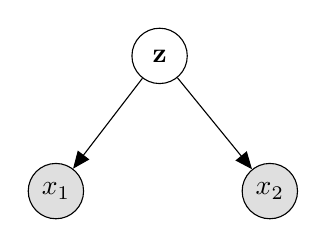
\begin{tikzpicture}
  % Define nodes
  \node[obs]                               (x1) {$x_1$};
  \node[obs, right=2cm of x1]              (x2) {$x_2$};
  \node[latent, above=of x2, xshift=-1.4cm] (z) {$\mathbf{z}$};
  % Connect the nodes
  \edge {z}{x1}  ; %
  \edge {z}{x2}  ; %
\end{tikzpicture}
  \\
  {\footnotesize The general notion is that taking projection onto the direction
  computed by CCA or PCA or GCCA is like computing the expectaion of
  the latent variable under the posterior distribution arrived at
  using the MLE estimates. The case for GCCA not published yet but
  highly plausible.}
\end{figure}
\end{frame}

\begin{frame}{Interpretations Of GCCA - Neural Net and Manifold}
\begin{enumerate}
\item Neural Adaptive CCA.
\item Adaptive CCA based on Matrix manifolds.
\end{enumerate}
\end{frame}

\begin{frame}{An application of GCCA.}
  Another formulation of the objective. $U_j = L_j$, $G = g$ from
  earlier notation.
  \begin{equation}
  \label{eq:gcca}
\begin{split}
  \operatorname*{\arg\,\min}_{G,U_j} & \sum_{j=1}^J \begin{Vmatrix} G - X_jU_j \end{Vmatrix}^2_F \\
  \text{such that } & G^\top G = I
\end{split}
\end{equation}
The solution is given by the following.
\begin{align}
P_j =& X_j(X_j^\top X_j)^{-1}X_j^\top \label{eq:pp}\\
M =& \sum_{j=1}^J P_j \label{eq:mm}\\
M G =& G \Lambda\\
U_j =& \left(X_j^\top X_j\right)^{-1} X_j^\top G
\end{align}
\end{frame}

\begin{frame}{An application of GCCA.}
  We used GCCA to extract dense representations/suficient statistics
  from word-word co-occurrence data.

  Consider that you mapped symbols from different sources to each other.
  
  \begin{displaymath}
    \xymatrix{
      A   & B   &  C  & \alpha & \beta & \gamma \\
      A   & B   &  C  & \beta & \beta & \gamma \\
      A   & B   &  C  & \le     &    \ge &   \neq   \\
          & A   &  C  & \le     &    \ge & \\ 
      C   & B   &  A  & \clubsuit & \diamondsuit & \heartsuit
    }
  \end{displaymath}
\end{frame}

\begin{frame}{Results - 1}
  \begin{table}[htbp]
  \resizebox{\textwidth}{!}{
  \begin{tabular}{=l +c +c | +c +c  +c +c }
    Test Set                             & Glove  & Word2Vec &
    \specialcell{MV-LSA\\(Monolingual)} & Gap & \specialcell{MV-LSA\\(All Views)}& $\Delta$      \\
MEN                                      & 71.0   &  73.9    & 70.7 & -3.2  & 71.1 & 0.4   \\
RW                                       & 28.5   &  32.9    & 26.4 & -6.5  & 37.1 & 10.7  \\
SCWS                                     & 54.5   &  65.6    & 60.4 & -5.2  & 66.5 & 6.1   \\
SIMLEX                                   & 33.0   &  36.7    & 32.3 & -4.4  & 40.3 & 8.0   \\
WS                                       & 59.2   &  70.8    & 70.3 & -0.5  & 71.1 & 0.8   \\
MTURK                                    & 62.2   &  65.1    & 55.9 & -9.2  & 58.9 & 3.0   \\
WS-REL                                   & 53.3   &  63.6    & 62.8 & -0.8  & 65.1 & 2.3   \\
WS-SIM                                   & 68.6   &  78.4    & 75.3 & -3.1  & 78.0 & 2.7   \\
RG                                       & 72.5   &  78.2    & 72.1 & -6.1  & 74.6 & 2.5   \\
MC                                       & 69.2   &  78.5    & 80.9 &  2.4  & 77.7 & -3.2  \\
TOMAS-SYN                                & 58.7   &  59.8    & 42.7 &-17.1  & 56.4 & 12.7  \\
TOMAS-SEM                                & 79.6   &  73.7    & 37.3 &-42.3  & 40.6 & 3.3   \\
 TOEFL                                   & 85.0   &  81.2    & 71.2 &-13.8  & 80.0 & 8.8  
  \end{tabular}
  }
  \caption{Comparison of Word2Vec, Glove and Multiview LSA.}
  \label{tab:c}
\end{table}
\end{frame}
\begin{frame}{Results - 2}
\begin{table}[htbp]
  \resizebox{\textwidth}{!}{
  \begin{tabular}{=l +c +c +c +c +c +c +c +c}
Test Set              & \specialcell{All\\Views} & !Framenet & !Morphology & !Bitext & !Wikipedia & !Dependency & \specialcell{!Morphology\\!Framenet} & \specialcell{!Morphology\\!Framenet\\!Bitext} \\
\hline
MEN                                   & 70.1     &  69.8    &   70.1       &  69.9   &   46.4       & 68.4     &    69.5   &    68.4     \\
RW                                    & 37.2     &  36.4    &   36.1       &  32.2   &   11.6       & 34.9     &    34.1   &    27.1     \\
SCWS                                  & 66.4     &  65.8    &   66.3       &  64.2   &   54.5       & 65.5     &    65.2   &    60.8     \\
SIMLEX                                & 41.1     &  40.1    &   41.1       &  37.8   &   32.4       & 44.1     &    38.9   &    34.4     \\
WS       & 69.4     &  69.1    &   69.2       &  67.6   &   43.1       & 70.5     &    69.3   &    66.6     \\
MTURK    & 58.4     &  58.3    &   58.6       &  55.9   &   52.7       & 59.8     &    57.9   &    55.3     \\
WS-REL   & 61.6     &  61.5    &   61.4       &  59.4   &   38.2       & 63.5     &    62.5   &    58.8     \\
WS-SIM   & 76.8     &  76.3    &   76.7       &  75.9   &   48.1       & 75.7     &    75.8   &    73.1     \\
RG       & 73.2     &  72.0    &   73.2       &  73.7   &   45.0       & 70.8     &    71.9   &    74.0     \\
MC       & 78.3     &  75.7    &   78.2       &  78.2   &   46.5       & 77.5     &    76.0   &    80.2     \\
TOMAS-SYN                             & 56.4     &  56.3    &   56.2       &  51.2   &   37.6       & 50.5     &    54.4   &    46.0     \\
TOMAS-SEM                             & 34.3     &  34.3    &   34.3       &  36.2   &   4.1        & 35.3     &    34.5   &    30.6     \\
TOEFL    & 82.5     &  82.5    &   82.5       &  71.2   &   45.0       & 85.0     &    82.5   &    65.0    
  \end{tabular}
  }
  \parbox{\textwidth}{\caption{Performance versus views removed from
      the multiview GCCA procedure. !Framenet means that the view
      containing counts derived from Frame semantic dataset was
      removed. Other columns are named similarly. The other
      hyperparameters were $n_j=\textrm{Count}^{\frac{1}{4}}, \;
      m=300, \; t=100K, \; v=25$. }}
  \label{tab:vj}
\end{table}

\end{frame}
\end{document}
